% !TEX encoding = UTF-8 Unicode
% !TEX root = project.tex

\documentclass{sig-alternate}
\usepackage{authblk}
\usepackage{url}
\usepackage{subfig}
\usepackage{amsmath}

\begin{document}

%don't want date printed
\date{}

\title{Is Your Code Noodle-free? \\
Predicting Defect-prone Areas Using Noodlr}

\author{Bastin Gomez Headmon}
\author{Vishal Chaudhary}
\affil{David R. Cheriton School of Computer Science, University of Waterloo}
\affil{\textit {\{bgheadmo,v3chaudh\}@uwaterloo.ca}}

\maketitle

% Use the following at camera-ready time to suppress page numbers.
% Comment it out when you first submit the paper for review.
\thispagestyle{empty}

\pagenumbering{arabic}

% !TEX encoding = UTF-8 Unicode
% !TEX root = project.tex

\subsection*{Abstract}

In a software development setup, resources are the most expensive component that are involved at every stage of the software development cycle. Allocating resources is a critical decision that is taken by the managers and the higher management. In making such a critical decision, one needs to have a good understanding of the system, its complexities and dependencies. At times, even though managers have good functional domain knowledge, they lack technical or product/software specific knowledge. Hence, knowingly or unknowingly, they take wrong decisions about allocating resources to the module which needs more attention, which affect the overall cost of the project. Maintenance is the stage in the software development cycle where the maximum time is spent and it is also the most expensive. Hence it needs the most optimized resource allocation. At this stage, wrongly allocated resources might affect overall budget of the project drastically. \\

For better decision making in above situations, we implemented a tool called Noodlr, which gives an insight of the source code repository and helps managers to make better decisions. Noodlr is an open dependency graph generator tool, implemented in D3.js~\cite{d3js} in the frontend and Java in the backend, shows the overall design and architecture of the project. Noodlr shows the most critical areas where the probability of getting defects is more using Kosaraju's strongly connected components algorithm~\cite{sharir1981strong}. Noodlr can be used in development, maintenance and testing stages of a software project. Noodlr can be also be used for training purposes to give an idea about the overall project structure and file dependencies.

\keywords{dependency graph, strongly connected components, maintenance, testing.}

% !TEX encoding = UTF-8 Unicode
% !TEX root = project.tex

\section{Introduction}
\label{sec:intro}
According to Gartner, global software expenditures for 2015 amounted to \$3.52 trillion, and forcasted to grow 0.6 \% to \$3.54 trillion in 2016\cite{gartner2016}.\\

In any large scale project, as the teams and team size increases, size of the source code repositories as well as the number of lines of code (LOC) increase slowly. As the repositories increase in size, dependencies amongst all the objects in the repository also increases. After a certain point of time, it becomes extremely difficult for developers and managers to track these repositories. \\

From developer's perspective, to make any changes to the code, they will have to look deep inside the repository to see effects of their changes. Many simple tools provide that service in a very orthodox way (plain text format). For example, in Eclipse, on using Open Call Hierarchy for a method, it gives a list of all the other methods from various classes that are calling this method. In small projects, this can be helpful but in large size projects, finding relevant method becomes a tedious task. \\

From manager's perspective, they need to understand the design and architecture of the project, and defect-prone critical areas in it, so that resource allocation can be easily done in a optimized way. Managers usually have strong domain knowledge but at times, they lack technical design and architectural knowledge. So, if they have to make any critical decisions (like resource allocation), lack of sufficient knowledge on product/software specific information might lead to bad results (under/over allocation of resources).\\

So, to help developers and managers, we implemented Noodlr, a web based tool which can be used with any source code repository to get a detailed view. Developers can use it to check the dependencies and relationships between various programming components (like classes, methods and packages). So, before a developer makes any change in the code with respect to a defect resolution, he/she can use this tool to check the side-effects on other objects, if any. Managers can use this tool to detect the most defect-prone areas and hence can do resource allocation appropriately. \\

Also, in large projects, teams focusing on different areas work together with lots of dependencies between them. Many a times, work allocation becomes a problem for managers as they are not sure as to which team a particular piece of work should be assigned. This tool can be used to create the module boundaries as well, which makes the manager's job of work allocation easier.\\

Noodlr is an interactive web based tool, implemented in D3.js with a Java-based backend, that constructs a dependency graph for a given repository and shows all the parent-child relations, static call-dependencies and strongly connected components (using Kosaraju-Sharir's algorithm\cite{sharir1981strong}). In this project, we have attempted to achieve the following objectives:
\begin{enumerate}
    \item Implement a web based tool which provides an interactive graphical user interface (GUI) to explore the whole source code repository.
    \item Finding areas in the source code repository where the probability of getting defects is high. We have used Kosaraju-Sharir algorithm and Bron-Kerbosch algorithm for this purpose.
    \item Evaluate the efficiency of Kosaraju-Sharir algorithm and Bron-Kerbosch algorithm on few well-known open source projects.
    \item Evaluate if Noodlr gives appropriate results using the above mentioned algorithms by comparing it to the files in Github pull requests that are related to issues.
\end{enumerate}

In section \ref{sec:algos}, we discuss two major algorithms that we have used in our tool to find the defect-prone areas. In section \ref{sec:related}, we provide the motivation behind our project by explaining some of the related works. Thereafter, we discuss the software implementation of Noodlr in section \ref{sec:setup} as well as the backend server that implements Kosaraju-Sharir and Bron-Kerbosch algorithm. In the evaluation covered in section \ref{sec:finding}, we present the experimental study that was conducted on open source github repositories. For our study, we used a medium sized repository called Retrofit (around 9000 LOC) from Square Inc, a large sized repository called Twitter4j (around 33000 LOC) maintained by an independent developer, a third repository named Guava (around 143000 LOC) from Google and a small repository named Scribejava (around 5000 LOC). The last 2 repositories were not used for our visualization purposes and were used only for evaluation. In section \ref{sec:threats}, we discuss few short comings of our tool that we found from our evaluation and also discuss few drawbacks of one of the algorithms. In section \ref{sec:practical}, we discuss some of the practical applications of our tool. In section \ref{sec:conclusion}, we discuss the future work related to our tool and finally conclude the paper.

\section{Terminologies and Algorithms}
\label{sec:algos}

We attempt to use a couple of graph algorithms for the purpose of detecting defect-prone areas in a software project. First we construct graphs from the class dependencies and the method dependencies in the project. To restrict the scope of our work, we concentrate only on projects that use Java\footnote{\url{https://www.oracle.com/java/index.html}} as the main programming language. The graph is constructed with classes or methods forming the vertexes of the graph and the relationship between classes or methods forming the edges between the vertexes. Once the graph is fully constructed, we try to find the strongly connected components (SCC) using Kosaraju's algorithm (a.k.a Kosaraju-Sharir algorithm). We also try to find out maximal cliques using Bron-Kerbosch algorithm. 

\subsection{Strongly connected components (SCC)}
In the mathematical theory of directed graphs, a graph is said to be strongly connected if every vertex is reachable from every other vertex. The strongly connected components of an arbitrary directed graph form a partition into subgraphs that are themselves strongly connected\footnote{\url{https://en.wikipedia.org/wiki/Strongly_connected_component}}. Figure~\ref{fig:scc_sample} shows a sample graph marked with strongly connected components.

\begin{figure}[h!]
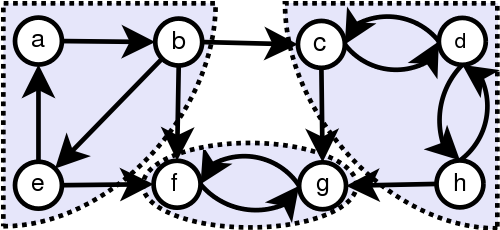
\includegraphics[width=8cm]{scc_sample}
\caption{SCC's marked in a sample graph}
\label{fig:scc_sample}
\end{figure}

\subsection{Kosaraju-Sharir algorithm}
Kosaraju-Sharir algorithm\cite{sharir1981strong} is a linear time algorithm to find the strongly connected components of a directed graph. Kosaraju's algorithm uses two passes of depth first search. The first pass is used to choose the order in which the outer loop of the second depth first search checks vertices for having been visited already and recursively explores them if not visited already. The second depth first search is on the transposed graph of the original graph, and each recursive exploration finds a new strongly connected component\cite{cormen2001introduction}.

\subsection{Maximal cliques}
A clique is a set of nodes in a graph where between every pair of nodes (X, Y) a dependency exists. A clique is maximal if no other node can be added without losing the clique property\cite{zimmermann2008predicting}. We attempt to find out maximal cliques from the graph constructed earlier and check whether it can be used for predicting the defect-prone areas of the project. To find the maximal cliques, we assume that the nodes in the graph is undirected. i.e., even though there is a direction in the dependency of classes or methods, for the purpose of finding maximal cliques, we let go of the direction of dependency.

\subsection{Bron-Kerbosch algorithm}
Bron-Kerbosch algorithm\cite{bron1973algorithm} is used to find maximal cliques in an undirected graph. We used the version of the algorithm which does not have pivoting. Although this algorithm is used in previous studies\cite{zimmermann2008predicting} to predict defect-prone areas, we were unsuccessful in our attempt to get any result by applying this algorithm on the software projects we selected. We conjecture that this may be due to the particular structure of the projects that we selected that did not have a maximal clique present in their structure.



% !TEX encoding = UTF-8 Unicode
% !TEX root = project.tex

\section{Related Work}
\label{sec:related}

In the past many authors and research institutes have focused their research work on finding defects and dependency graphs. \\

One of the most significant work was done by Thomas Zimmerman et al.~\cite{zimmermann2008predicting}, who tried to predict defects using network analysis on dependency graphs. The authors claimed that models using network analysis on dependency graphs to find defects proved to have better recall of around 10\% points higher than other models that used complexity metrics. Also, they proved that dependency graphs can help in finding around 60\% of critical areas, twice as identified by any other counterparts. Authors in this paper used, along with many other algorithms, Bron-Kerbosch's algorithm, which uses size of clique to determine the number of defects in that region. Their claim is that as the size of the clique grows, its binaries become more defect-prone. Finally, they found that the average number of defects increases with the size of the clique a binary resides in. Figure~\ref{fig:relatedwork} and Figure~\ref{fig:relatedwork1} shows a glimpse of what the Bron-Kerbosch is aimed at and how the results will look like, respectively. In our study and implementation, we tried to implement Bron-Kerbosch algorithm, but we could not get any meaningful results on the projects that we tried.

\begin{figure}[h!]
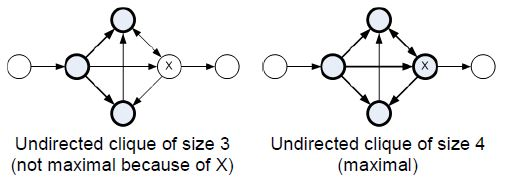
\includegraphics[width=8cm]{relatedwork}
\caption{Undirected cliques}
\label{fig:relatedwork}
\end{figure}

\begin{figure}[h!]
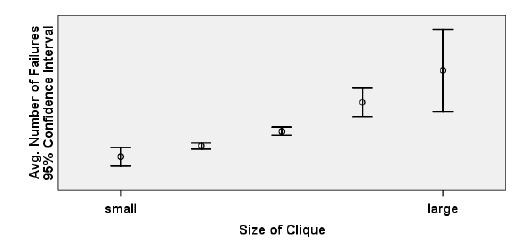
\includegraphics[width=8cm]{relatedwork1}
\caption{Defect-Proneness of binaries in cliques}
\label{fig:relatedwork1}
\end{figure}

Our evaluation section follows similar steps as implemented in the paper that we just mentioned. In our evaluation, we performed an experimental study that attempted to use 2 major algorithms, Kosaraju-Sharir and Bron-Kerbosch's algorithm to find the defect-prone areas in the source repositories. Although we were unsuccessful with Bron-Kerbosch algorithm, we managed to get some results out of the implementation of Kosaraju-Sharir algorithm. Later, the Noodlr tool shows the strongly connected components on the graph obtained using the Kosaraju-Sharir algorithm. Results are discussed in more detail in the evaluation section (Section~\ref{sec:finding}). \\

Another study~\cite{bhattacharya2012graph} done by the researchers of the Department of Computer Science, University of California - Riverside discusses the recent advancements in analysis of graph topology to make the understanding of software evolution more clear. Also, they tried to create predictors that can help in software development and maintenance. In this study, they demonstrated how graph based analysis can be used in software evolution by estimating bug severity, prioritizing re-factoring efforts and also predict defect-prone releases. As compared to this, Noodlr also helps in various stages of software development including development, testing and maintenance stages which are discussed in detail in Practical Applications (Section~\ref{sec:practical}). \\

At 34\textsuperscript{th} Euromicro Conference Software Engineering and Advanced Applications~\cite{turhan2008software}, a paper was published on predicting software defects using Call Graph Based Ranking (CGBR). In this study, authors claimed to use static call graph based ranking along with a defect prediction model. Though the results show that CGBR framework could get the same number of defective modules as other counterparts, it produced very low false alarm rates. In their evaluation study, they proved that testing process can be improved by 23\% through CBGR framework. This study proposed a novel combination of the static code attributes (SCA) and architectural structure of software to make predictions about defect content of software modules.\\

A slight variant of ~\cite{turhan2008software} in this area is presented in~\cite{eichinger2008mining}. Authors of the paper~\cite{eichinger2008mining} tried to solve the problem of automating the discovery of non-crashing occasional bugs. They claimed that mining of weighted call graphs of program executions could be a good way to automate this. In their model, they proposed a novel reduction technique for call graphs which introduces edge weights on each link. Then this weighted graph is used for analysis to find bugs. Evaluation provided some bugs which were not detected by any other previous studies and even the precision of finding localised bug doubled compared to any other prior studies.\\

A recent study on telecommunication industry~\cite{turhan2009data} that includes mining source code using data mining techniques for locating software bugs was presented in Elsevier 2009 conference. The paper focused on similar objectives like our paper to help managers in resource allocation and testing by predicting defect-prone areas in large-sized projects. They followed an approach similar to the CBGR methodology as discussed in ~\cite{turhan2008software}. Results of this paper suggested that, at least 70\% of the defects can be detected by inspecting only 6\% of the code using a Naive Bayes model and 3\% of the code using CGBR framework.\\

Now, in the next section, we look at the actual software implementation of the frontend and the backend. We explain how the above mentioned algorithms are used in the software as well as how the data is presented in the Noodlr interface, which is our web-based tool.



% !TEX encoding = UTF-8 Unicode
% !TEX root = project.tex

\section{Software Implementation}
\label{sec:setup}
\\
In this section, we would like to explain the implementation of Noodlr including the frontend and backend of the tool. Since Noodlr is a web based tool, we have divided this section into two namely:
\begin{enumerate}
    \item Noodlr frontend implementation
    \item Noodlr backend implementation
\end{enumerate}

Frontend can be accessed from anywhere with the help of a web browser that has Javascript enabled. For evaluation purposes, we used a laptop with Intel Core i7-2720QM CPU running at 2.2 GHz with 8 GB RAM, with Windows 7 professional operating system.\\

For the backend, implementation was done on a single laptop having an Intel Core i5 CPU running at 1.6 GHz with 4 GB RAM, with OSX El Capitan operating system.

\subsection{Frontend Implementation}
Noodlr was envisioned to be an interactive web based tool, so we decided to make use of JavaScript language to implement the front end of Noodlr. Since the objective of Noodlr was to provide an interactive interface which can be used by managers and developers, the interface was developed in D3.js\cite{d3js}. D3.js (D3 = Data-Driven Documents) is a JavaScript library for producing dynamic, interactive data visualizations in web browsers. It makes use of the widely implemented SVG, HTML5, and CSS standards. D3 provides hundreds of data visualization options, but our motive was to incorporate a style which can display the graph of packages, classes and methods showing the parent-child relationship (to show Package-Class and Class-method) as well as showing links with source and targets arrows (to show call dependencies). \\

A popular D3 style called Sankey style\footnote{\url{http://bl.ocks.org/wvengen/cab9b01816490edb7083}} was a good choice as per our requirement, as we wanted to have an expand-and-collapse functionality for our graph nodes. For example, if user double clicks on a class node, it should expand and draw all the method nodes and if he/she again double clicks on the top left corner on the particular class node, all its method nodes should collapse into one class node. We had to make changes in the Sankey D3 library to create this expand and collapse functionality.\\

In our design, every component(class, method and package) has a node with a different colour on the graph. All the package nodes contains class nodes embedded and all the class nodes contain the method nodes embedded. If user double clicks on the package (with green colour node), an animation will be shown with the package moving to the top left corner of the browser window and all the contained classes will pop out on the graph with orange colour nodes. If user double clicks on the class (with orange colour node), an animation will be shown with the class node moving to the top left corner and it will pop out all the methods on the graph (with violet colour nodes). Similarly, top left corner nodes which were created by the earlier actions can be double clicked to collapse related nodes on the graph.\\

Our custom Sankey style takes two JSON files as input. One file is the parent-child relationship file, with each node defined with various attributes in key-value pair form. For example, a class Class1 is defined as follows:

\begin{table}[h]
    \centering
    \begin{tabular}{lll}
        \{\\
        ``type'' & : & ``Class'',\\
        ``id'' & : & ``c1'',\\
        ``parent'' & : & ``p1'',\\
        ``name'' & : & ``Class\_1'',\\
        ``full\_name'' & :& ``p1.Class\_1''\\ 
        \}
    \end{tabular}
    \caption{\textbf{JSON node type 1}}
    \label{tab:node1}
\end{table}
  
 JSON node as shown in Table~\ref{tab:node1} states that this node is of type class, with id `c1' whose parent is package `p1' and name of this node is `Class\_1'. In this way, all packages, classes and methods are defined in a JSON file. Second file contains the links with source and target nodes defined in another JSON format. Format shown in Table~\ref{tab:node2} is of that JSON file.

\begin{table}[h!]
    \centering
    \begin{tabular}{lll}
        \{\\
        ``source'' & : & ``m1'',\\
        ``target'' & : & ``m2'',\\
        ``value'' & : & ``calls / depends on'',\\
        \}
    \end{tabular}
    \caption{\textbf{JSON node type 2}}
    \label{tab:node2}
\end{table}

In the JSON node shown in Table~\ref{tab:node2}, the source id and the target id are defined, with the kind of relationship they share as the value. For example, in the JSON node shown in Table~\ref{tab:node2}, method `m1' calls method `m2' and hence making a link on the graph. After these two input files are available, Noodlr calls custom Sankey style D3 library and renders the D3 graph on the user's screen.\\\\
From the Noodlr following properties can easily be observed:


\begin{table}[h]
\centering
\begin{tabular}{ll}
\hline
Property & Description\\
\hline
Shape & State of the node (Expanded/Collapsed)\\
Color & Type of node (Package, Class \& Method)\\
Height & Amount of linkages\\
Arrows & Caller to called node\\
Hovered text & Node description\\
\hline
\end{tabular}
\caption{Different measures \& their description in Noodlr.}
\label{tab:prop1}
\end{table}\\

To explain the properties shown in Table~\ref{tab:prop1}, we would like to use Figure \ref{fig:noodlr_ui}. As can be seen in Figure~\ref{fig:noodlr_ui}, Class\_1 is connected with Class\_2 and Class\_3 where Class\_1 method is calling some method of Class\_2 and a method of Class\_1 is calling a Class\_3 method. 

\begin{figure}[h!]
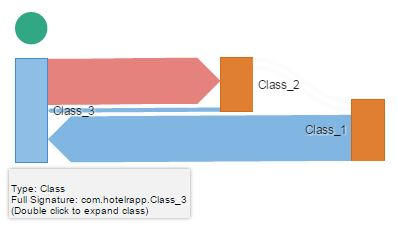
\includegraphics[width=8cm]{measures}
\caption{Noodlr User Interface}
\label{fig:noodlr_ui}
\end{figure}

\begin{enumerate}
    \item \textbf{Shape}: All the expanded nodes can be seen in the top left corner in circular shape. All the collapsed nodes are shown in a rectangular shape. In Figure~\ref{fig:noodlr_ui}, green coloured circle represents a package that contains Class\_1, Class\_2 and Class\_3.
    \item \textbf{Color}: Green represents `Package', Orange represents `Class', Violet represents `Method' and Light blue color represents hovered node.
    From arrows perspective, Red colored arrow represents current hovered node that is calling the other node at the target end of the arrow. Whereas the Light blue arrow represents current node being called by other node which is at the source end of the arrow.
    \item \textbf{Height}: Height of each rectangular node represents the number of links with respect to other nodes in the graph. Larger height of node means more links with other nodes in the graph.
    \item \textbf{Arrows}: Arrows play a vital role in Noodlr. Arrows represent which Node is calling/depends on which other node. Arrow's source is the caller node and target is the called node.
    \item \textbf{Hovered text}: Hovered text is used extensively in Noodlr and is used on each component. If any node is hovered, the hovered text shows some main characteristics like type, full signature and the action to be taken. On arrows, hovered text explains which node is calling which other node.
\end{enumerate}


Figure~\ref{fig:noodlr_ui_package} shows how the open call hierarchy graph visualization will look like for a small project when the nodes are all collapsed. We have selected a small project to make it easier to demonstrate in the limited space of the paper. In this view, it shows all the Java packages of the project. Since this is a small sample project, there are classes in the the project which are not in any Java packages, i.e., in the default package. That is shown as ``DEFAULT'' package in the figure. When all the packages represented by the green nodes are double-clicked, the image shown in Figure~\ref{fig:noodlr_ui_class} will show up. That is a partially expanded view where it shows the relationships between the Java classes in the project. This view can be further expanded to show up the methods present in the classes and their relationships. This view is shown in Figure~\ref{fig:noodlr_ui_method}. This is the completely expanded view of the graph and the highest granularity possible with the tool. A user can choose to expand only those packages of his interest and to see how relationships emerge from there. In all these 3 representations, the user can hover on any node to see all the nodes that it connects to and the detailed description of the node.


\begin{figure}[h!]
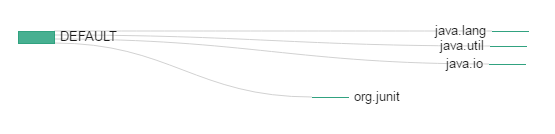
\includegraphics[width=8cm]{ui-package-view}
\caption{Noodlr UI: Package view (Fully collapsed)}
\label{fig:noodlr_ui_package}
\end{figure}

\begin{figure}[h!]
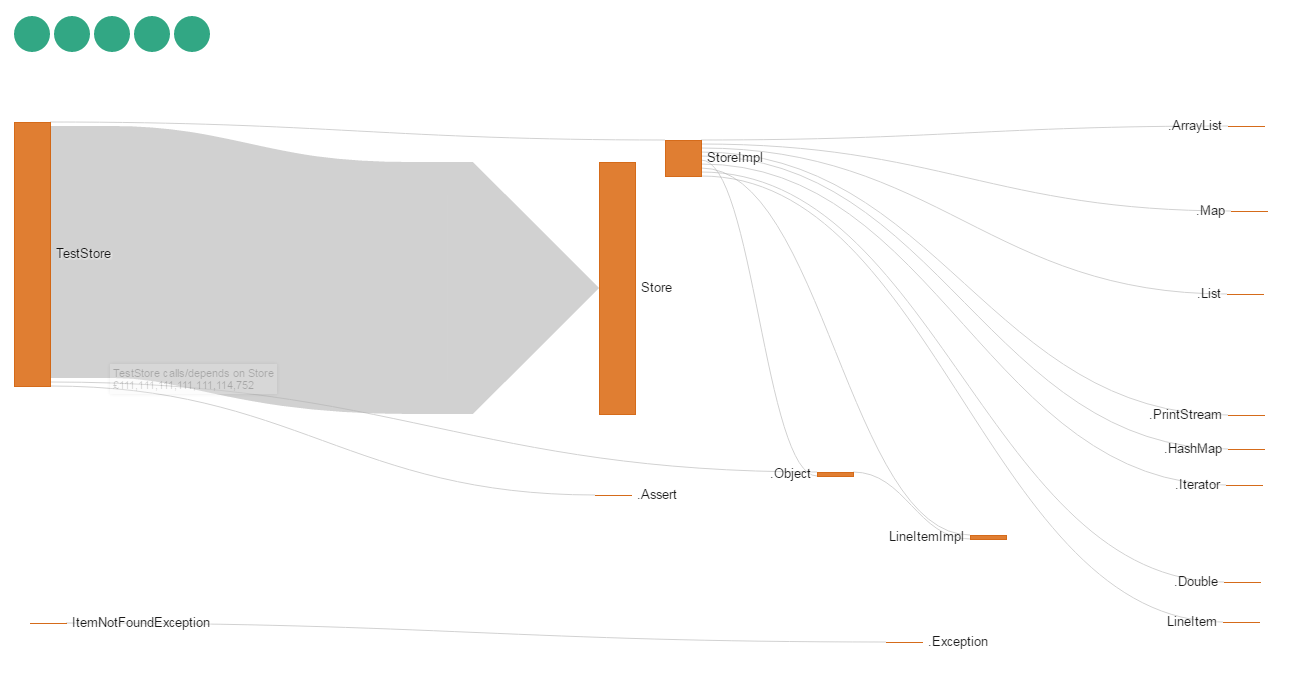
\includegraphics[width=8cm]{ui-class-view}
\caption{Noodlr UI: Class view (Partially expanded)}
\label{fig:noodlr_ui_class}
\end{figure}

\begin{figure}[h!]
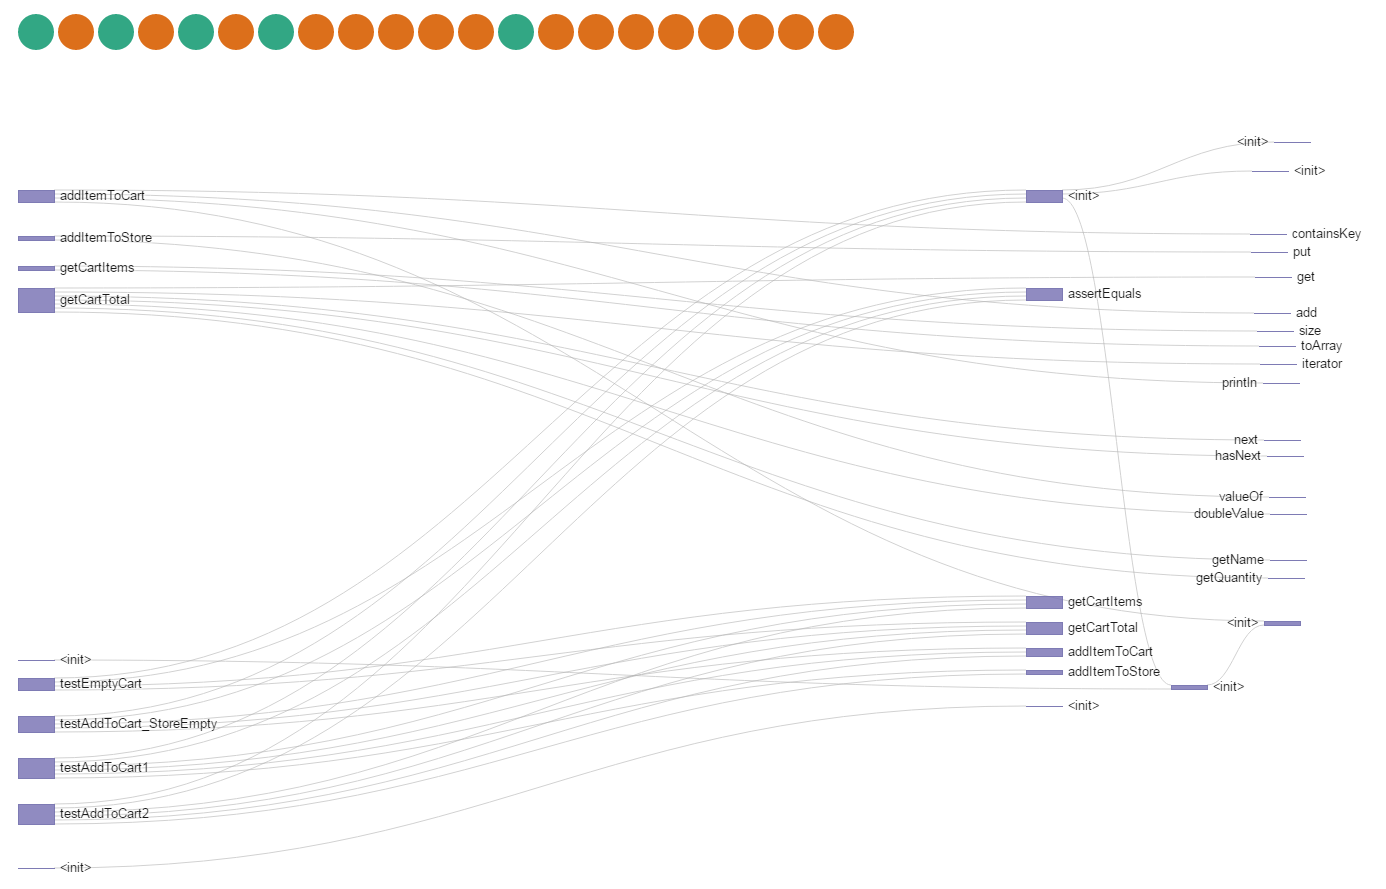
\includegraphics[width=8cm]{ui-method-view}
\caption{Noodlr UI: Method view (Fully expanded)}
\label{fig:noodlr_ui_method}
\end{figure}

\subsection{Backend implementation}

The backend implementation was done in Java and contains the logic to read the project files and create the graph of packages, classes and methods. Once the graph is generated, various graph algorithms such as the Kosaraju-Sharir algorithm and the Bron-Kerbosch algorithm were applied. This was to generate parts of the graph which is more defect-prone than others.\\

The first part of the process was to read an input jar file. Although there were multiple options to read files from a project, taking jar file as input seemed to be a straightforward choice for us given that the jar files are generated after the project is cleanly build without errors. Once the jar file is read, it is searched for class files and all class files are read using Apache Commons Byte Code Engineering Library (Apache Commons BCEL\texttrademark). All the methods are also read and their dependencies found along with the class to class dependencies. Using all the class to class dependencies and the method to method dependencies found using BCEL, a graph is constructed with vertexes as the classes or methods and edges as the relationship between them. \\

Once the graph was constructed, we implemented the required algorithms in Java to work on the graph to produce required results. The output produced by the Java implementation of the algorithms were fed to the frontend to produce the D3 graphs which could be displayed to the user.


% !TEX encoding = UTF-8 Unicode
% !TEX root = project.tex

\section{Evaluation}
\label{sec:finding}

In order to evaluate the effectiveness of our tool, we ran experiments on existing projects in GitHub. We only selected Java-based projects as we used Java specific tools to generate static call hierarchies. We wrote a script in Ruby\footnote{\url{https://www.ruby-lang.org/en/}} which could download the source code associated with pull requests\footnote{\url{https://help.github.com/articles/proposing-changes-to-a-project-with-pull-requests/}} using the Github API\footnote{\url{https://developer.github.com/v3/}}. The retrieved pull request information and the associated file information were saved into a set of database tables for further analysis. Then we further filtered the list down to make sure that only issue related pull request files were considered. This data was compared against the strongly connected components data obtained by running our implementation of the Kosaraju-Sharir algorithm, which was also used for populating the front-end user interface. This comparison would give us an idea of how helpful our tool would have been, in retrospect. 

\subsection{Evaluation Setup}

We gathered data from 4 projects in GitHub: Guava~\cite{guava}, Retrofit~\cite{retrofit}, Twitter4j~\cite{twitter4j} and Scribejava~\cite{scribejava}. The project descriptions are listed in Table \ref{tab:evaluationprojects}. The main programming language used in these projects is Java. From these small sample set of data that we evaluated against, our tool was able to successfully predict (recall) 36\%, 66\%, 5\% and 14\% respectively for the projects Guava, Twitter4j, Retrofit and Scribejava. 

\begin{table}[h]
\centering
\begin{tabular}{ll}
\hline
Project & Description \\
\hline
Guava & Google Core Libraries for Java \\
Retrofit & Type-safe HTTP client \\
Twitter4j & Java library for the Twitter API \\
Scribejava & Simple OAuth library for Java \\
\hline
\end{tabular}
\caption{Projects used for evaluation.}
\label{tab:evaluationprojects}
\end{table}

All of these open source GitHub projects had several pull requests and a lot of these pull requests were created for issues. One of the criterion that we used to select projects from Github is that they are not new projects which tend to have less number of pull requests and they may not be helpful for our experiments. Another criterion is to have a fair number of pull requests and a good mix of java files in them. Third criterion is that they can be packaged to form a jar file which our tool consumes. Although it was an option for us to implement the tool which could accept a project folder, it made more sense for us to package it as a jar file, which contained class files after building the project.

\subsection{Evaluation Results}

For the Guava project, we only took the core module which itself gave a good sized project to work on. We found 817 files using our tool that is part of the strongly connected components of the project and is predicted to be more defect-prone. But only 143 files were retrieved from the pull request of the corresponding module. When we matched these files, we found that 52 files were common between these two sets. That gave us a recall of 36\%, i.e., 52 out of 143 files. With respect to precision, only 52 out of 817 files were correct, i.e., only 6\% precision for the Guava project.

\begin{figure}[h!]
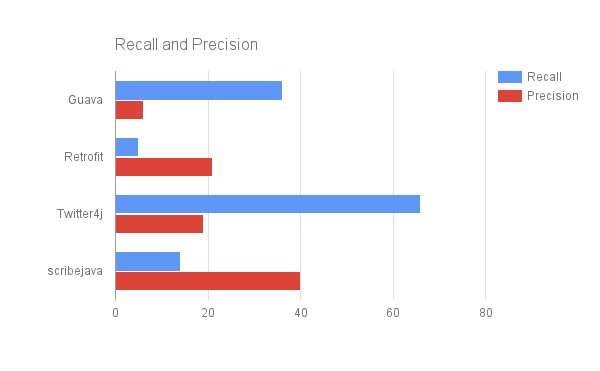
\includegraphics[width=8cm]{recall-precision}
\caption{Bar chart showing values of precision and recall}
\label{fig:precision_recall}
\end{figure}

The second project that we analysed was Retrofit. The tool predicted that 55 files were more defect-prone from the strongly connected components calculation. From the data we obtained from Github for this project, there were 214 files. Only 12 files were found to be common between these sets. That gave us a recall of 5\% (i.e., 12 out of 214 files) and a precision of 21\% (i.e., 12 out of 55 files).\\

The third project that we analysed was Twitter4j, in which we took only the core module which was big enough for our analysis. A total of 245 files were predicted to be defect-prone by the tool based on its strongly connected component calculation. 72 files were obtained from the Github repository for the project which were part of the pull requests. We found that there are 48 files which are common between these two sets. So the recall came out to be 66\% (48 out of 72 files) and precision calculated was 19\% (48 out of 245 files).\\

The last project that we analysed was Scribejava, and we took only the core module. This was comparatively a smaller project as compared to the other ones. A total of 25 files were predicted by the tool to be defect-prone based on the module's strongly connected components. 73 files were obtained from the Github repository for the project which were part of the pull requests. 10 files were found to be common between these two sets. That made the recall to be 14\% (10 out of 73 files) and the precision to be 40\% (10 out of 25).\\

Figure~\ref{fig:precision_recall} shows the graphical representation of the precision and recall obtained for projects that we took for analysis. Scribejava project has the highest value for Precision (40\%) and second lowest value for Recall (14\%).\\

There were no patterns that emerged from these figures, the reason for which we conjecture is because of the varied number of pull requests and the files associated with them. One project had a lot more files associated with them forming more number of strongly connected components. More experimental studies would be required to come out with a good explanation for these figures.\\

\begin{figure*}[h!]
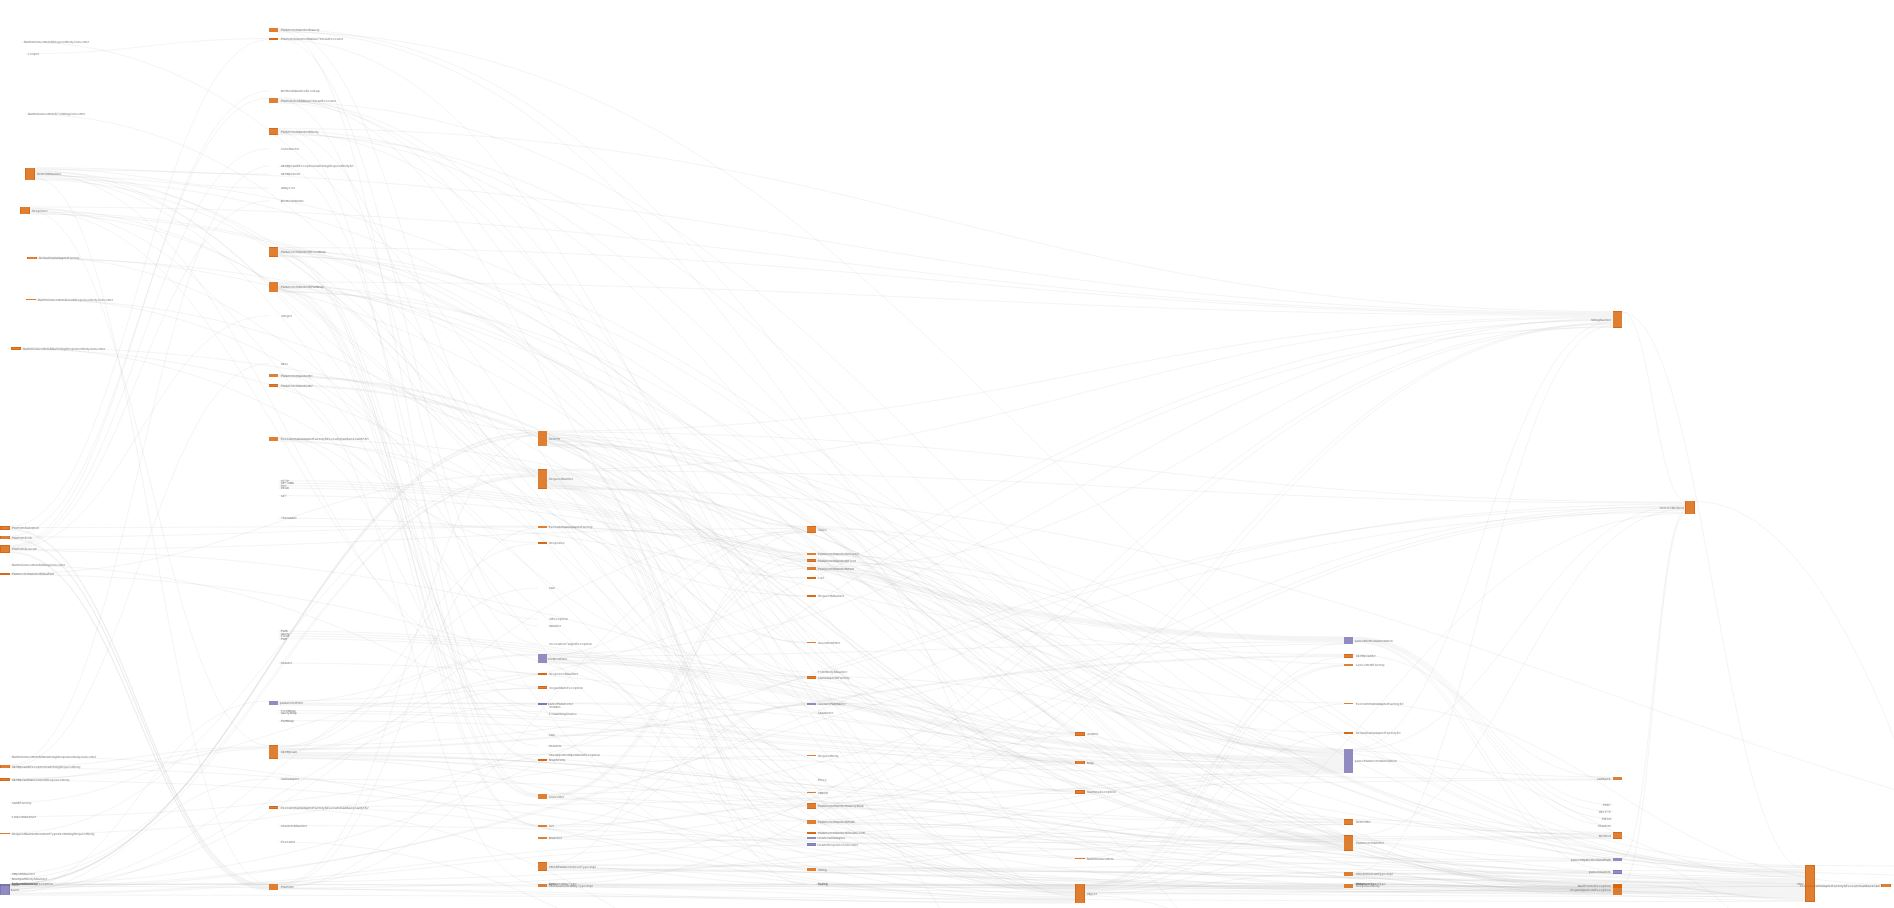
\includegraphics[width=16cm]{graph}
\caption{Noodlr dependency graph for a medium sized project}
\label{fig:graph}
\end{figure*}

\subsection{Threats to Validity}
\label{sec:threats}

\subsubsection{Small Sample Set}

The sample size of pull requests that we used for evaluation is quite small. Although we wrote a script in Ruby\footnote{\url{https://www.ruby-lang.org/en/}} to query Github to extract pull requests using their API, we were limited to manually inspect the pull request data for candidate matches rather than writing a tool to mine this data automatically. This limitation was due to the short amount of time that we had for this project. Future work may include authoring a tool that would effectively mine this data from GitHub and verify the usefulness of our tool in a more efficient manner. Also, even though we gathered data from 4 different projects, we are not claiming that this data is representative of all types of software projects. The 4 projects differ in size and their applicability and also in the number of files available in the pull requests. With a larger sample set of test data that spans several more projects, we would be able to get a better idea of the effectiveness of our tool.

\subsubsection{Developer Behaviors}

All developers are different and with that, most developers have different behaviors. Related to the small sample set limitation described above, we cannot avoid the possibility of using data where the developer behaved in an abnormal manner. For instance, it is completely possible that a developer may have checked-in a large number of files from different part of the project which are not related and the relations between these files would eventually emerge at a later point of time. In this sense, the tool will not be able to predict those files because they are not part of strongly connected components. Our tool does not take this behavior into account as it solely looks at the files belonging to strongly connected components.

\subsubsection{Types of Changes Made}

From exploring hundreds of pull requests, we have noticed that there are several types of software changes that are made where our tool may be more applicable. Generally, for changes that are made where the modifications are in a focused area of a system where components are strongly connected, such as a sub-system component where all parts of the component are related in some way. However, for changes that span a wide area of seemingly unrelated components, or changes such as general comment additions, or spelling corrections, or those things which are unrelated to the Java source files it is difficult for our tool to predict adequately.


\subsubsection{Limitations on D3.js design}

D3 is a open source library which is improved through continuous support of design and data visualization community. For our project also, we had to make some changes in the project to make the Sankey style more interactive with the user. Similarly, there are many other changes that are required in our UI. Most basic issue with current UI of Noodlr is that it cannot support huge projects efficiently. Since the expansion of each node creates many more new child nodes, the screen size becomes an issue after a point. It can be seen in Figure~\ref{fig:graph}, where a medium size project makes it very hard for the user to explore as users will have to scroll and zoom to get a better picture.

\subsubsection{Restriction in the programming language used}

Our tool, in its current state, will work only with projects that use Java as the main programming language. We used tools such as Apache Commons Byte Code Engineering Library (Apache Commons BCEL\texttrademark) for extracting the static call hierarchies. This restricts the scope of our tool. In order to support a new programming language, we will be required to implement language specific tools which can provide us with static call hierarchies. Though, this logic of extracting call hierarchies is a high-level idea that can be used in any programming language, the applicability is severely dependent on the availability of such tools for that programming language. 


% !TEX encoding = UTF-8 Unicode
% !TEX root = project.tex

\section{Practical Applications}
\label{sec:practical}
We envisioned our tool to help employees of an organization who are at different functional levels such as managers, developers, testers et.al. Some of the practical applications of our tool as follows:

\subsection{For resource allocation purposes}
\label{sec:resource_allocation}

For managers, it is of great help if he knows where to allocate more resources for development and testing. Our tool will give a birds-eye view of the different components in the applications such as packages, classes and methods. It also gives a good idea about the critical sections of the application. Due to the interactive nature of the tool, the manager can select only a particular portion of the application if required and highlight them to get a detailed view.

\subsection{For internal training purposes}
Usually large size projects have so many different teams and repositories, it becomes really hard to teach technical project design and architecture to new joiners. Even though senior developers try to give a clear explanation using everything they have, it is very hard for the new joiner to understand it completely and clearly. Noodlr can help in this regard immensely. Noodlr can be used for training new joiners in the project and show them the overall design of the whole project. It can also be used to demonstrate the usage of each package, class and method as well and how different classes and methods interact with each other to provide required services in the product.

\subsection{For tracking defect-prone areas}
As already discussed in above sub section \ref{sec:resource_allocation}, as the size of the repository increases, it becomes very difficult for the managers to allocate resources efficiently. Noodlr can help managers in providing an insight of the most defect-prone areas in the repository and then, managers can allocate resources accordingly. 

\subsection{Development stage: Track dependencies}
From developers point of view, many a times it becomes extremely hard to use available tools to check call dependencies. For example, Open Call Hierarchy functionality in Eclipse editor is very helpful for developers. But, as the size of the repository grows, it becomes extremely difficult to explore the whole list, especially when that method is being used vastly across the whole project. In this scenario, Noodlr can help developers to see all the call dependencies around a particular method or class. Using Noodlr, developer can focus on call dependencies in a particular focused domain (e.g. inside the package, class etc) as well.
\subsection{Maintenance stage: Change existing code}
As a developer, Noodlr is most useful in Maintenance stage of a development cycle. To fix a particular defect, developers can see the call dependency graph and create an estimate of the effects that he might face after implementing the change. In this way, many a times developer will not have to test randomly as he/she can see its drastic effects on the other dependencies. This way, Noodlr improves the productivity of the developer.
\subsection{Testing Stage: Make regression testing plan}
Good testers never ignore any possible scenarios where a bug is expected. Noodlr can help testers to create better test cases and test plans based on the dependency graph. As all the affected dependencies can be seen clearly in Noodlr UI, testers can create extra test cases in their regression batch job to make sure that all the dependencies are tested again after every change.

\section{Conclusion}
\label{sec:conclusion}

Maintaining the high quality of a software system is a difficult task, especially for systems where there are several contributors. It becomes even more hard as the size of the project increases. Managers face an increasingly difficult task of assigning resources to the right focus area based on its complexity. They face the challenge of upholding a high level of quality given the number of developers that have the right knowledge to work on these systems. We presented the Noodlr tool that helps managers, developers and testers gain a detailed understanding of the system in terms of the various components of the system and their inter-dependencies. We developed the Noodlr tool as a web-based tool which does not require any installation to use and is user-friendly, interactive and intuitive. We evaluated the validity of our work by testing our tool against several project samples from Github and found that it produces results with reasonable precision and recall. Our hope is that this work will help people from different functional levels in their ability to function better.\\

\subsection{Future Work}
\label{sec:future}
In this work, visualizing projects with size more than a particular limit was difficult as it created a very dense graph with D3's custom Sankey style. As an improvement in future, we would like to use another style or even a different visualization library to make the user experience seamless irrespective of the size of the project. \\

Currently, we have not implemented a search functionality for files, packages, methods or any other items in the project being visualized. As a future enhancement, we would like to implement a full-fledged search feature in this tool. \\

Currently the support is limited to Java based projects as we are using tools that only work with Java. We would like to incorporate support for projects that are written in other programming languages in future.\\

We would also like to integrate our tool as a plugin into different IDEs such as Eclipse\footnote{\url{https://eclipse.org/}}, Intellij Idea\footnote{\url{https://www.jetbrains.com/idea/}}, Netbeans\footnote{\url{https://netbeans.org/}} et.al.



%% !TEX encoding = UTF-8 Unicode
% !TEX root = project.tex

\section{Acknowledgments}
This section is optional; it is a location for you
to acknowledge grants, funding, editing assistance and
what have you.  In the present case, for example, the
authors would like to thank Gerald Murray of ACM for
his help in codifying this \textit{Author's Guide}
and the \textbf{.cls} and \textbf{.tex} files that it describes.

%
% The following two commands are all you need in the initial runs of your .tex file to produce the bibliography for the citations in your paper.
\bibliographystyle{abbrv}
\bibliography{project} 

%% !TEX encoding = UTF-8 Unicode
% !TEX root = project.tex

%APPENDICES are optional
%\balancecolumns
\appendix
%Appendix A
\section{Headings in Appendices}
The rules about hierarchical headings discussed above for
the body of the article are different in the appendices.
In the \textbf{appendix} environment, the command
\textbf{section} is used to
indicate the start of each Appendix, with alphabetic order
designation (i.e. the first is A, the second B, etc.) and
a title (if you include one).  So, if you need
hierarchical structure
\textit{within} an Appendix, start with \textbf{subsection} as the
highest level. Here is an outline of the body of this
document in Appendix-appropriate form:
\subsection{Introduction}
\subsection{The Body of the Paper}
\subsubsection{Type Changes and  Special Characters}
\subsubsection{Math Equations}
\paragraph{Inline (In-text) Equations}
\paragraph{Display Equations}
\subsubsection{Citations}
\subsubsection{Tables}
\subsubsection{Figures}
\subsubsection{Theorem-like Constructs}
\subsubsection*{A Caveat for the \TeX\ Expert}
\subsection{Conclusions}
\subsection{Acknowledgments}
\subsection{Additional Authors}
This section is inserted by \LaTeX; you do not insert it.
You just add the names and information in the
\texttt{{\char'134}additionalauthors} command at the start
of the document.
\subsection{References}
Generated by bibtex from your ~.bib file.  Run latex,
then bibtex, then latex twice (to resolve references)
to create the ~.bbl file.  Insert that ~.bbl file into
the .tex source file and comment out
the command \texttt{{\char'134}thebibliography}.
% This next section command marks the start of
% Appendix B, and does not continue the present hierarchy
\section{More Help for the Hardy}
The sig-alternate.cls file itself is chock-full of succinct
and helpful comments.  If you consider yourself a moderately
experienced to expert user of \LaTeX, you may find reading
it useful but please remember not to change it.
%\balancecolumns % GM June 2007
% That's all folks!	

\end{document}
